\section{Contexte}
En l'état actuel, lorsque les pompiers doivent intervenir dans le cas d'un incident impliquant des fuites d'hydrocarbures sur route, la répartition
du produit absorbant se fait via une remorque-semoirs. Celle-ci dispose de trois sections de dépose de produit qui sont télécommandées directement par un opérateur.
Durant l'intervention, une personne doit marcher à côté de la remorque afin d'observer et contrôler la répartition du produit, nous pouvons relever les points suivant:
\begin{enumerate}
    \item L'opérateur doit marcher, cela limite la vitesse du véhicule et les longues distances sont problématiques.
    \item La détection se fait à l'oeil nu, l'opérateur doit donc rester concentrer en permanence au risque de devoir repasser sur certaines zone.
    \item La commande est manuelle, il est possible de faire des erreurs sur la commande risquant la dépose de surplus de produit ou de devoir repasser sur certaines zone.
\end{enumerate}
\textbf{Le but de se travail de Bachelor est d'automatiser ce processus, via un système de détection des hydrocarbures par vision industrielle et d'un pilotage de l'ouverture/fermeture des vérins.}
\section{Cahier des charges \label{cdc}}
Le cahier des charges est le suivant:
\begin{itemize}
    \item Préparer un planning détaillant les tâches.
    \item Définir un setup permettant de:
          \begin{itemize}
              \item Analyser les traces d'hydrocarbures selon leur positionnement sur la route.
              \item Commander la télécommande du semoir.
          \end{itemize}
    \item Sélectionner les éléments composant le setup.
    \item Commander les éléments.
    \item Assembler les éléments.
    \item Tester le setup et procéder aux ajustements nécessaires.
    \item Développer un logiciel d'analyse et de gestion de la télécommande.
    \item Tester le logiciel d'analyse et de gestion de la télécommande.
    \item Valider le logiciel et le comportement sur la route.
    \item Analyser et interpréter les résultats.
\end{itemize}
\section{Planning}
Le planning vient compléter le cahier des charges du chapitre \ref{cdc} en ajoutant le travail à effectuer pour chaque étape ainsi qu'une estimation
de l'effort à fournir en heure.

Le planning ci-dessous présente les étapes, le détail des sous-étapes, l'effort à fournir estimé ainsi que la période durant laquelle chaque étape sera présumément effectuée (en bleu).
\begin{figure}[H]
    \centering
    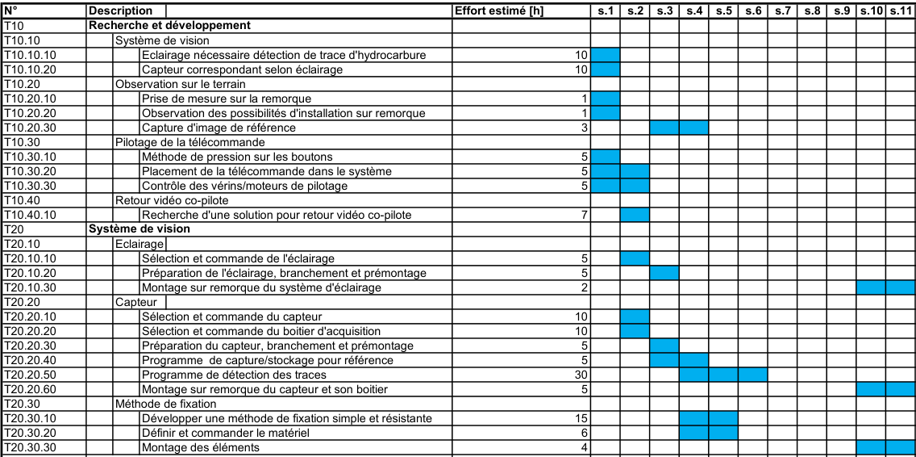
\includegraphics[width=15cm, angle=90]{assets/figures/planning1.png}
    \caption{Planning - partie 1}
\end{figure}
\newpage
\begin{figure}[H]
    \centering
    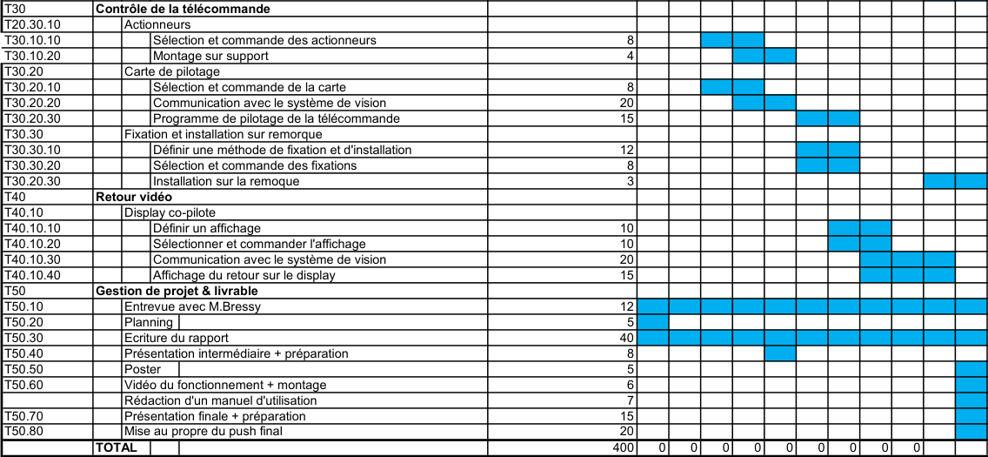
\includegraphics[width=15cm, angle=90]{assets/figures/planning2.png}
    \caption{Planning - partie 2}
\end{figure}

En complément au planning ci-dessus, on peut imaginer une vingtaine d'heures d'imprévus supplémentaires.